\section{安装运行}

\subsection{运行 Ollama}

\begin{frame}[fragile]
\frametitle{运行 Ollama}
\textbf{启动 Ollama 服务}
\begin{lstlisting}
export OLLAMA_MODELS=/usr/share/ollama/.ollama/models
export OLLAMA_HOST=0.0.0.0
export OLLAMA_SCHED_SPREAD=1
export CUDA_VISIBLE_DEVICES=0,1,2,3,4,5,6,7

nohup sh -c 'ollama serve' > ollama.log 2>&1 &
\end{lstlisting}
\begin{itemize}
    \item \textbf{注意}:
    \begin{itemize}
        \item \texttt{OLLAMA\_HOST} 必须设置为 \texttt{0.0.0.0},否则后续 Open Webui 无法访问 Ollama。
        \item \texttt{OLLAMA\_SCHED\_SPREAD} 必须设置为 \texttt{1},否则无法多卡运行单一模型。
    \end{itemize}
\end{itemize}
\end{frame}

\begin{frame}[fragile]
\frametitle{拉取 DeepSeek R1}
% \subsection{拉取 DeepSeek R1 模型}
\textbf{使用 Ollama 拉取 DeepSeek R1 模型}
\begin{lstlisting}
ollama pull deepseek-r1:671b # 默认就是 q4_K_M 量化
\end{lstlisting}
\end{frame}

\subsection{使用 Open Webui 对话}
\begin{frame}
\frametitle{使用 Open Webui 对话}
% \subsubsection{Open Webui 配置}
\textbf{Open Webui 后端地址设置}
\begin{figure}
    \centering
    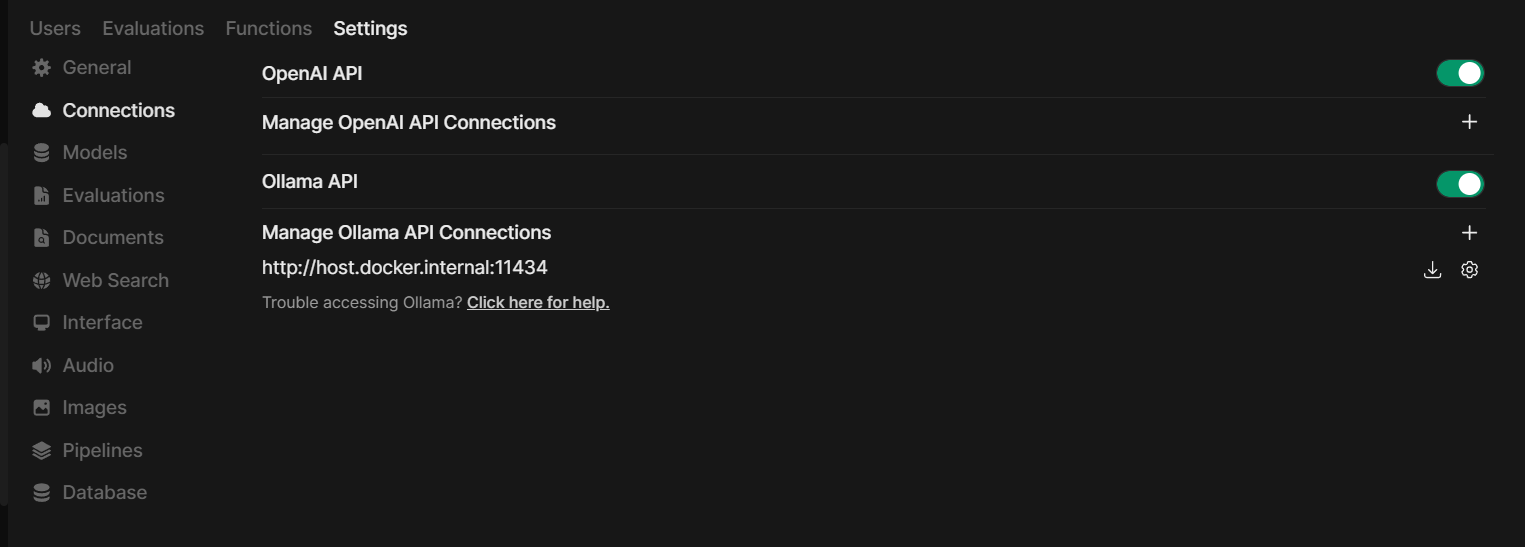
\includegraphics[width=\textwidth]{./pic/1.png} % 替换为你的图片路径
    % \caption{Open Webui 后端地址设置示例}
    \label{fig:openwebui_backend}
\end{figure}
% \textit{图片来源: \url{https://raw.githubusercontent.com/Lanthanum1/my_images/main/img/202502112050602.png}} % 图片来源注释
\end{frame}

\begin{frame}
\frametitle{Open Webui 配置详解}
% \subsubsection{Open Webui 配置详解}
\begin{itemize}
    \item Open Webui 配置分三层:模型级, 账户级, 聊天级。
    \item 优先级: 模型级 > 账户级 > 单次聊天级。
    \item \textbf{单次聊天级 (Per-Chat)}: 聊天右侧 Chat Controls 中设定,仅对当前会话生效,不能覆盖模型预设。
    \item \textbf{模型级 (Per-Model)}: Admin Panel-Settings-Models 中设定,适用于所有使用该模型的聊天,优先级最高。
    \item \textbf{账户级 (Per-Account)}: Settings-Advanced Parameters 中设定,会被模型级配置覆盖。
\end{itemize}
\end{frame}

\begin{frame}
\frametitle{Open Webui 调整参数}
% \subsubsection{Open Webui 性能调优}
\begin{itemize}
    \item 8 卡 A100 在设定Context Length和Max Tokens都为8k后可正常推理,每张卡显存占用约为50-60GB.
    \item 默认情况下,5min内如果没有新的对话,模型会从 GPU 中 offload,重新加载至显存需要很长时间。可以在 Settings-Advanced Parameters 中设定 Keep Alive 参数,设为 -1 则用不卸载。
    \item  如果显存不够,可通过设置 \texttt{num\_gpu} 参数来灵活调整 CPU/GPU 推理比例。
        \begin{itemize}
            \item 例如设为 \texttt{60} 则 60 层加载到 GPU,剩余在 CPU 推理。
        \end{itemize}
		\item 完成上述配置后,即可在 Open Webui 中与 DeepSeek R1 模型进行对话。
\end{itemize}
\end{frame}

% \begin{frame}
% \frametitle{Open Webui 对话}
% % \subsubsection{开始对话}
% \begin{itemize}
    
% \end{itemize}
% \end{frame}	